\documentclass[12pt]{article}

\usepackage[T1]{fontenc} \usepackage[icelandic]{babel}
\usepackage[margin=0.5in]{geometry}
\usepackage{latexsym,amssymb,amsmath}
\usepackage{pgfplots}
\usepackage{float}
\usepackage[absolute,overlay]{textpos}
\newcounter{marknumber}
\pgfplotsset{
    error bars/every nth mark/.style={
        /pgfplots/error bars/draw error bar/.prefix code={
            \pgfmathtruncatemacro\marknumbercheck{mod(floor(\themarknumber/2),#1)}
            \ifnum\marknumbercheck=0
            \else
                \begin{scope}[opacity=0]
            \fi
        },
        /pgfplots/error bars/draw error bar/.append code={
            \ifnum\marknumbercheck=0
            \else
                \end{scope}
            \fi
            \stepcounter{marknumber}    
        }
    }
}
\usepackage{graphicx}
\graphicspath{ {./} }
\usepackage{hyperref, color}
\hypersetup{
    colorlinks=true,
    linktoc=all,
    linkcolor=blue,
}
\usepackage{tikz}
\usetikzlibrary{decorations.pathreplacing,calligraphy}

\begin{document}
    
\centerline{\bf \Huge EÐL207G Lokaskýrsla}
\centerline{\bf \large Bylgueiginleikar Ljóss}
\centerline{\bf Torfi Þorgrímsson}

\tableofcontents
\newpage

\section{Inngangur}

Í þessari tilraun er skoðað bylgju eiginleika ljóss. Þetta er gert með einlitum laser sem er skínt í gegnum raufar, í kringum hár og í gegnum skautunarsíur. 

Ljós er bylgja. Meira nákvæmlega er ljós orku pakki sem ferðast í gegnum rafsegulsviðið sem bylgja, þar sem helmingur er rafbylgja og hinn er segulbylgja. Þetta gefur ljósi ákveðna eiginleika sem við getum hannað tilraunir til að skoða. 

\subsection{Sundrun}

Eiginleikin sem við notum í fyrstu þrem tilraunum okkar er ljóssundrun. Ljóssundrun gerist þegar ljós rekst í hlut og sundrast í allar áttir. Hinsvegar sundrast það ekki eins mikið í allar áttir. 

% Skíringar mynd 1
\begin{center}
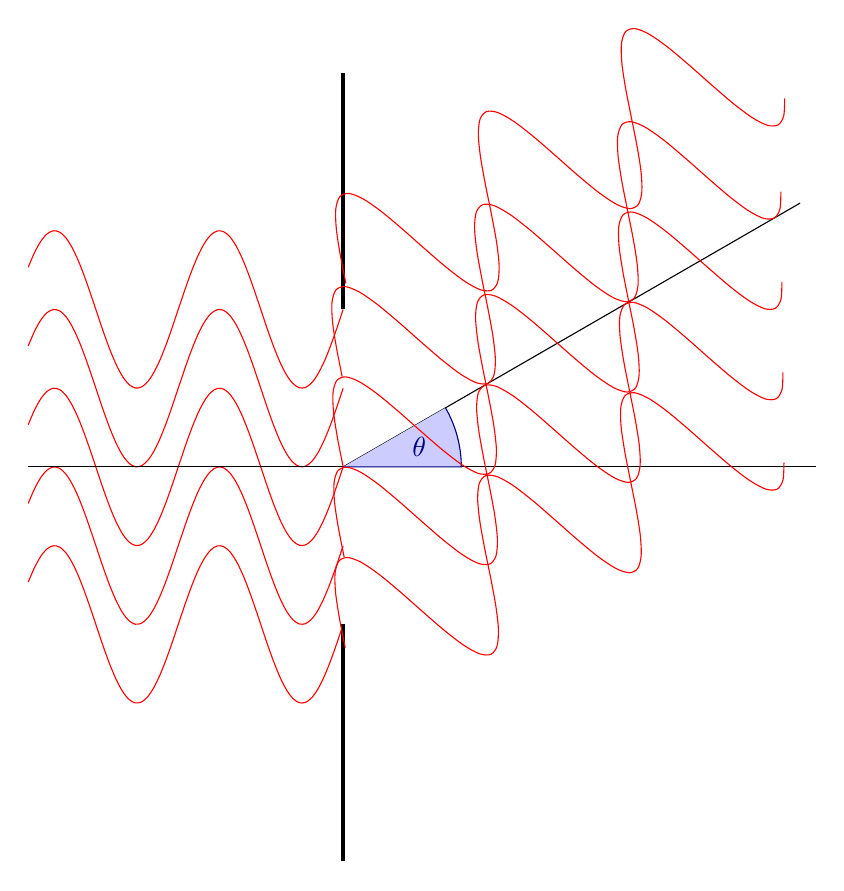
\begin{tikzpicture}[ declare function={f1(\x)=sin(3*deg(\x));}]
    \begin{scope}[local bounding box=T]
        \draw[color=red] plot[domain=-4:0,variable=\x,samples=51,smooth] 
            ({\x},{f1(\x)+2});
        \draw[color=red] plot[domain=-4:0,variable=\x,samples=51,smooth] 
            ({\x},{f1(\x)+1});
        \draw[color=red] plot[domain=-4:0,variable=\x,samples=51,smooth] 
            ({\x},{f1(\x)});
        \draw[color=red] plot[domain=-4:0,variable=\x,samples=51,smooth] 
            ({\x},{f1(\x)-1});
        \draw[color=red] plot[domain=-4:0,variable=\x,samples=51,smooth] 
            ({\x},{f1(\x)-2});
    \end{scope}
    
    \draw[ultra thick] (0,-5) -- (0,-2);
    \draw[ultra thick] (0,5) -- (0,2);

    \draw (-4,0) -- (6,0);
    \draw (0,0) -- (30:6.7);

    
    \filldraw[fill=blue!20,draw=blue!50!black] (0,0) -- (1.5,0) arc(0:30:1.5);
    \draw (15:1) node[blue!50!black] {$\theta$};

    \begin{scope}[local bounding box=T]
        \draw[color=red,rotate=30,right=34] 
            plot[domain=0:6,variable=\x,samples=51,smooth] 
                ({\x},{f1(\x)+2});
        \draw[color=red,rotate=30,right=16] 
            plot[domain=0:6,variable=\x,samples=51,smooth] 
                ({\x},{f1(\x)+1});
        \draw[color=red,rotate=30,right=00] 
            plot[domain=0:6,variable=\x,samples=51,smooth] 
                ({\x},{f1(\x)});
        \draw[color=red,rotate=30,left=16] 
            plot[domain=0:6,variable=\x,samples=51,smooth] 
                ({\x},{f1(\x)-1});
        \draw[color=red,rotate=30,left=32] 
            plot[domain=0:6,variable=\x,samples=51,smooth] 
                ({\x},{f1(\x)-2});
    \end{scope}

\end{tikzpicture}

\bf Skýringar mynd 1.

{\footnotesize Skoðum eina átt af sundruðu ljósi}

\end{center}

Til að skylja hvað gerist þegar ljós sundrast í allar áttir skoðum við aðeins einn bita af því sem er allt að fara í sömu átt, eins og sést á skýringar mynd 1. Á myndinni sjáum við ljós bylgju með samhliða bylgjutoppa koma frá vinstri átt og hitta rauf og hinumegin við raufina skoðum við aðeins ljósið sem fer í áttina $\theta$, og við sjáum að bylgju topparnir eru ekki lengur samsíða, þannig að þeir munu eiða og styrkja hvorn annan. Við getum líka ímyndað okkur hvað gerist ef við breytum áttini sem ljósið fer, og við getum valið okkur heppilegt horn þar sem bylgjurnar aðeins styrkja eða aðeins eiða hvort öðrum. Við hvaða horn ljósið styrkist eða eyðist er háð raufar stærðinni og bylgjulengd ljóssins.

Ef við skýnum sundraða ljósinu á vegg, þá lítur ljósstyrkurinn út eins og Teikning 1. En ef við bætum við annari rauf þá mun ljósið sundrast frá báðum raufum styrkja eða eiða hvort öðrum og þá lítur ljósstyrkurinn út eins og Teikning 2. 

% Teikningar 1&2
\begin{center}
    \includegraphics[scale=0.5]{html/teikning1.png}
    \includegraphics[scale=0.5]{html/teikning2.png}
    
    \bf Teikning 1.
    \qquad
    \qquad
    \qquad
    \qquad
    \bf Teikning 2.

    {\footnotesize Ein rauf}
    \qquad
    \qquad
    \qquad
    \qquad
    \quad
    {\footnotesize Tvær raufar}

\end{center}

\subsection{Skautun}

Ljós er mjög líkt bylgju á vatni, nema að ljós sveiflast frjálst í tveim víddum, ámeðan vatnsyfirborðsbylgjur sveiflast næstum bara í einni vídd, upp og niður. Áttin sem ljósið sveiflast er kallað skautun ljóssins. Þegar við sendum ljós í gegnum skautunarsíu þá síum við í burtu það ljós sem er ekki skautað í sömu átt og sían. 

Ef ljós fer í gegnum síu sem er ekki skautuð í sömu át þá getum við hugsað okkur að ljósið sé samansett af tveim ljóseindum, ein sem er skautuð með síunni og hin skautuð $90^\circ$ á móti síunni, sem ef lagðar saman gefa upprunulegu ljóseindina. Aðeins sá partur sem er skautaður með síunni kemst í gegn og hinn er stoppaður. Þannig að ef við sendum ljós í gegnum tvær síur með skuatunarmun af $90^\circ$ þá ætti ekkert ljós að komast í gegn.


\section{Lýsingar}

Hér næst munum við útskýra allar tilraunirnar og tilgang þeirra.

\subsection{Tilraun 1: Mæling bylgjulengd ljóss}

% Skíringar mynd 2
\begin{center}
\begin{tikzpicture}[scale=3,rotate=90]
	\def\Lone{1.06417777}
	\def\Ltwo{1.30540728}

	\draw [decorate, decoration = {calligraphic brace}] (0,1) -- (70:\Lone);
	\draw (80:1.13) node {$x_1$};
	\draw [decorate, decoration = {calligraphic brace}] (130:\Ltwo)  -- (0,1);
	\draw (110:1.23) node {$x_{-2}$};

	\draw (-1,1) -- (1,1);

	\filldraw[fill=green!20,draw=green!50!black] (0,0) -- (0,3mm) arc(90:70:3mm);
	\draw (80:2.5mm) node[green!50!black,scale=0.5] {$\theta_1$};
	\filldraw[fill=blue!20,draw=blue!50!black] (0,0) -- (0,4mm) arc(90:130:4mm);
	\draw (118:3.2mm) node[blue!50!black,scale=0.5] {$\theta_{-2}$};

	\draw [decorate, decoration = {calligraphic brace}] (0,0) -- (0,1);
	\draw (-0.08,0.5) node[scale=0.5] {$L$};

	\draw[red] (0,0) -- (70:\Lone);
	\draw[red] (0,0) -- (110:\Lone);
	\draw[red] (0,0) -- (130:\Ltwo);
	\draw[red] (0,0) -- (50:\Ltwo);
	\draw[red] (0,0) -- (90:1cm);

    \draw[] (-0.5,0) -- (-0.003,0);
    \draw[] (0.003,0) -- (0.5,0);
	\draw (0.6, 0) node[scale=1] {$d_r=1880 nm$};
    \draw[red] (0,0) -- (0,-1);
    \draw[thick] (-0.5,-1) -- (-0.004,-1);
    \draw[thick] (0.004,-1) -- (0.5,-1);
    \draw (0.6,-1) node[scale=1] {Þykkt takmarkari};
    \draw[thick,red] (0,-1) -- (0,-2);
	\draw (-0.1,-2) node[right=1cm,above=0.5mm] {Laser} rectangle (0.1,-3);
\end{tikzpicture}

\bf Skýringa mynd 2.

{\footnotesize Uppsetning tilraun 1.}

\end{center}

Á skýringa mynd 2 sést hvernig tilraun 1 var uppset; Laser er skotin í rauf til að minka geislann fyrir betri mælingu, svo fer laserinn í gegnum mjög mjóa rauf sem hefur vídd sem við vitum frá framleiðanda, $1880nm$. Næst sjáum við geisla sem merkja sterkustu hluta ljóssins, sem eru þá bylgju topparnir á teikningu 1, með þeim munum við reikna bylju lengd ljóssins, því við höfum mjög þægilega jöfnu sem að lýsir þessari uppsetningu.

\[d_r \sin{\theta} = m\lambda\]

Þar sem $d_r$ er vídd raufarinnar, $\theta$ er áttin sem geislinn fer, $m$ er númer geislanns og $\lambda$ er bylgjulengdin.

\subsection{Tilraun 2: Mæling bil á milli raufa}

% Skíringar mynd 2
\begin{center}
\begin{tikzpicture}[scale=3,rotate=90]

    \draw (-1,1) -- (1,1);

    \draw[color=red,rotate=90] plot[domain=0:1,variable=\x,samples=51,smooth] ({\x},{\x*0.5});
    \draw[color=red,rotate=90] plot[domain=0:1,variable=\x,samples=51,smooth] ({\x},{\x*0.4});
    \draw[color=red,rotate=90] plot[domain=0:1,variable=\x,samples=51,smooth] ({\x},{\x*0.3});
    \draw[color=red,rotate=90] plot[domain=0:1,variable=\x,samples=51,smooth] ({\x},{\x*0.2});
    \draw[color=red,rotate=90] plot[domain=0:1,variable=\x,samples=51,smooth] ({\x},{\x*0.1});
    \draw[color=red,rotate=90] plot[domain=0:1,variable=\x,samples=51,smooth] ({\x},{\x*0});
    \draw[color=red,rotate=90] plot[domain=0:1,variable=\x,samples=51,smooth] ({\x},{\x*-0.5});
    \draw[color=red,rotate=90] plot[domain=0:1,variable=\x,samples=51,smooth] ({\x},{\x*-0.4});
    \draw[color=red,rotate=90] plot[domain=0:1,variable=\x,samples=51,smooth] ({\x},{\x*-0.3});
    \draw[color=red,rotate=90] plot[domain=0:1,variable=\x,samples=51,smooth] ({\x},{\x*-0.2});
    \draw[color=red,rotate=90] plot[domain=0:1,variable=\x,samples=51,smooth] ({\x},{\x*-0.1});

    \draw[] (-0.5,0) -- (-0.003,0);
    \draw[] (-0.0015,0) -- (0.0015,0);
    \draw[] (0.003,0) -- (0.5,0);
    \draw (0.6, 0) node[scale=1] {$d$};
    \draw[red] (0,0) -- (0,-1);
    \draw[thick] (-0.5,-1) -- (-0.004,-1);
    \draw[thick] (0.004,-1) -- (0.5,-1);
    \draw (0.6,-1) node[scale=1] {Þykkt takmarkari};
    \draw[thick,red] (0,-1) -- (0,-2);
    \draw (-0.1,-2) node[right=1cm,above=0.5mm] {Laser} rectangle (0.1,-3);
\end{tikzpicture}

\bf Skýringa mynd 3.

{\footnotesize Uppsetning tilraun 2.}

\end{center}

Tilraun 2 er mjög lík tilraun 1, nema það að laserinn fer núna í gegnum tvær raufar, og þannig fáum við fleiri bylgju toppa eins og á teikningu 2. Núna gyldir sama jafna og í tilraun 1 nema við skrifum $d$ sem bilið á milli raufa, en ekki $d_r$ vídd raufa.

\[d \sin{\theta} = m\lambda\]

\subsection{Tilraun 3: Mæling þykkt hárs}

Tilraun 3 er eins og tilraunir 1 og 2 nema við setjum mannshár fyrir framan laserinn og við skrifum $a$ í stað $d$ eða $d_r$ til að merkja þykkt hársins. Við sjáum svo að við fáum sama styrkmynstur eins og í teikningu 1.

\[a \sin{\theta} = m\lambda\]

\subsection{Tilraun 4: Mæling styrk ljóss í gegnum skautunarsíu}

% mynd 1
\begin{center}
    \includegraphics[scale=0.4]{html/polMynd.jpg}
    {\scriptsize https://www.vision-systems.com/cameras-accessories/article/14092924/polarization-definition-of-concepts-techniques-technologies}
    
    \bf Mynd 1.

    {\footnotesize Sýning á hvernig skautunarsíur virka}
\end{center}

Núna sendum við laserljós í gegnum tvær skautunarsíur við mismunandi skuatunarmun og mælum styrk ljóssins við hvern skuatunarmun. Út af þríhyrningafræði búumst við við að styrkurinn fylgi þessari jöfnu:

\[ I = I_0 \cos^2{\psi} \]

Þar sem $I$ er styrkur ljóssins, $I_0$ er mesti styrkur ljóssins (þegar síurnar beina í sömu átt) og $\psi$ er skuatunarmunurinn.

Við mælum styrk ljóssins með rafrænum mæli sem sendir straum eftir hve sterkt ljósið er, og þannig mælum við styrk ljóssins í Amperum.

\section{Útreikningar og gröf}

\subsection{Tilraun 1}

\[d_r \sin{\theta} = m\lambda\]

Til að finna út hvað $\lambda$ er þurfum við að finna út hvað $\sin{\theta}$ er. Léttasta leiðin til að gera það er að mæla rétthyrnda þríhyrninginn með hliðarnar $L$ og $x_n$ eins og sést á skýringar mynd 2. Til að finna $\theta$ vitum við að:

\[x_n^2+L^2=\text{langhlið}^2 \Rightarrow \sin{\theta}=\dfrac{x_n}{\text{langhlið}}=\dfrac{x_n}{\sqrt{x_n^2+L^2}}\]

Við vitum líka að við getum reiknað óvissu á útreikning með mörgum breytum með formúlunni:

\[\Delta y = \sqrt{\left(\dfrac{\partial y}{\partial x_1} \Delta x_1\right)^2+\left(\dfrac{\partial y}{\partial x_2} \Delta x_2\right)^2 + \cdots }\]

Og þá fáum við að óvissan á $\sin \theta$ er:

\[\Delta\sin\theta=\sqrt{\left(\dfrac{\partial\sin\theta}{\partial x_n} \Delta x_n\right)^2+\left(\dfrac{\partial\sin\theta}{\partial L} \Delta L\right)^2}=\dfrac{L\sqrt{(L\Delta L)^2+(x\Delta x)^2}}{\sqrt{(x^2+L^2)^3}}\]

Og með þessu vitum við að hallatalan af Grafi 1 er $\lambda / d_r$

% Graf 1
\begin{center}
    \includegraphics[scale=0.5]{html/data_01.png}

    \bf Graf 1.
\end{center}

Við finnum hallatöluna með formúlunni:
$\lambda = d_r*\dfrac{\sin{\theta_{-2}}-\sin{\theta_{2}}}{(-2)-2} $

Óvissan á $\lambda$ hefur sama hlutfall og 
$\Delta (\sin{\theta_{-2}}-\sin{\theta_{2}})=\sqrt{(\Delta \sin{\theta_{-2}})^2-(\Delta \sin{\theta_{2}})^2}$.

Með $d_r=1880nm$ og $L = 9cm$ fáum við að $\lambda=711 \pm 4 nm$

\subsection{Tilraun 2}

Hér eru útreikningarnir þeir sömu nema við vitum $\lambda$ og ekki $d$, og lengdin $L$ er núna jafnt og $310 cm$

Við gerum tilraunina með tveim mismunandi raufum.

Fyrsta gefur:

\begin{center}
    \includegraphics[scale=0.5]{html/data_02.png}

    \bf Graf 2.
\end{center}

$d = 200 \pm 130 \mu m$
Framleiðandi gefur $250 \mu m$

Önnur gefur:

\begin{center}
    \includegraphics[scale=0.5]{html/data_03.png}
    
    \bf Graf 3.
\end{center}

$d = 500 \pm 150 \mu m$
Framleiðandi gefur $500 \mu m$

Óvissan er hlutfalslega stærri vegna þess að það sem við erum að mæla er minna.


\subsection{Tilraun 3}

En og aftur, sama stærðfræði, nema við höfum $a$ í stað $d$.

\begin{center}
    \includegraphics[scale=0.5]{html/data_04.png}
    
    \bf Graf 4.
\end{center}

Og við fáum $a=67\pm 2 \mu m$

Við vitum ekki hvaðan hliðrunin kemur í miðjuni á grafinu.

\subsection{Tilraun 4}

Loks komum við að einhverju nýju. Skautun ljóss.

\begin{center}
    \includegraphics[scale=0.5]{html/data_05.png}
    
    \bf Graf 5.
\end{center}

Á grafi 5 sjáum við gögnin í bláu og líkanið í rauðu. Líkanið er reiknað útfrá hæsta styrk sem var mældur eftir að laserinn fór í gegnum síurnar.

\section{Niðurstöður}

Frá öllu þessu höfum við grætt betri skilning á ljósi og hvernig það er hægt að nota það. 

Frá Tilraun 1, 2 og 3 lærðum við hvernig er hægt að mæla litla hluti með ljósi. Og Frá Tilraun 4 hvernig ljós hegðar sér þegar það fer í gegnum skautunar síu.


\end{document}